\documentclass[12pt,letterpaper]{article}

\usepackage[utf8]{inputenc}
\usepackage[T1]{fontenc}

\usepackage[margin=2.5cm,headheight=30pt,headsep=0.6cm]{geometry}
\usepackage{graphicx}
\usepackage{xcolor}
\usepackage{enumitem}
\usepackage{fancyhdr}
\usepackage{setspace}
\usepackage{amsmath}
\usepackage{tikz}
\usetikzlibrary{positioning}
\usepackage{caption}
\usepackage[hidelinks]{hyperref}

\renewcommand{\figurename}{Figura}
\renewcommand{\contentsname}{Índice}
\setstretch{1.15}
\setlength{\parindent}{0pt}
\setlength{\parskip}{0.7em}
\captionsetup{font=small,labelfont=bf}

% --- Encabezado y pie de página -------------------------------------------
\pagestyle{fancy}
\fancyhf{}
\lhead{\includegraphics[height=0.9cm]{img/image5.jpg}\ \textbf{TuBus}}
\cfoot{\footnotesize Plataforma de Movilidad Inteligente basada en el Estándar GTFS y Telemetría en Tiempo Real \hfill \thepage}
\renewcommand{\headrulewidth}{0.4pt}
\renewcommand{\footrulewidth}{0.4pt}

% --- Títulos con numeración manual (igual que el documento original) -------
\newcommand{\seccion}[1]{%
  \section*{#1}\addcontentsline{toc}{section}{#1}}
\newcommand{\subseccion}[1]{%
  \subsection*{#1}\addcontentsline{toc}{subsection}{#1}}

\begin{document}

% ===================== PORTADA ============================================
\thispagestyle{empty}
\begin{center}
  \includegraphics[width=\textwidth]{img/image1.png}\\[2cm]
  \includegraphics[height=3.2cm]{img/image2.jpg}\\[1.5cm]
  {\fontsize{34}{40}\selectfont \textbf{TuBus}}\\[1cm]
  \begin{minipage}{0.85\textwidth}
    \centering\large
    TuBus es un ecosistema tecnológico basado en dispositivos IoT y tecnología GTFS
    para monitorear rutas de transporte público en tiempo real, optimizando
    frecuencias y reduciendo tiempos de espera para los usuarios de la ciudad.
  \end{minipage}\\[2.5cm]
  {\large
  Brandon Rodriguez Senac\\
  José Daniel Medrano Ibarra\\
  Inzunza Ramírez Fidel Omar\\
  Salomé Landeros Salazar}
\end{center}
\newpage

% ===================== ÍNDICE =============================================
\begingroup\setlength{\parskip}{0.2em}\setstretch{1.0}\tableofcontents\endgroup
\newpage

% ===================== 1. RESUMEN =========================================
\seccion{1. Resumen}

El transporte público enfrenta una severa crisis bajo el modelo fragmentado
<<hombre-camión>>, causando que su uso caiga a solo el 19--22\% de los viajes
diarios. Cuantitativamente, el 50\% de los usuarios carece de información de
rutas, el 56\% percibe una mala relación costo-calidad y el 34.7\% se siente
inseguro (Implan Culiacán, 2020, p.~15).

Este proyecto surge para resolver la profunda insatisfacción ciudadana y la
baja rentabilidad de los concesionarios. Nuestra hipótesis plantea que un
ecosistema tecnológico escalable revertirá esta tendencia sin requerir
infraestructura gubernamental multimillonaria. La solución, <<TuBus>>, aborda
esta oportunidad mediante un modelo dual: una plataforma \textit{Software as a
Service} (SaaS) con dispositivos IoT de bajo costo instalados en los autobuses
para monitorear desviaciones, conectada a una aplicación móvil gratuita
impulsada por el estándar de datos abiertos GTFS (SEDATU \& GIZ, 2024, p.~12).

Las técnicas empleadas abarcan desde investigación de mercados ---con encuestas
que se aplicarán para validar la intención de adopción, estimada en más del
83\% por el Implan Culiacán (2020)--- hasta el modelado de arquitecturas de
telemetría. Se espera que los hallazgos confirmen la viabilidad de la
digitalización para recuperar la confianza del usuario. Los resultados
esperados incluyen la optimización de las frecuencias, la reducción de los
tiempos de espera y la transición gradual al cobro electrónico. En conclusión,
TuBus demuestra que modernizar el transporte desde el sector privado es
factible y urgente. Esta propuesta es pertinente con los ejes transversales de
Sostenibilidad Ambiental e Inclusión Social. Al incentivar el transporte masivo
frente al automóvil privado, se mitigan significativamente las emisiones de
carbono, y simultáneamente se democratiza el derecho a una movilidad urbana
segura, predecible y equitativa para toda la población (Mapasin, 2025, p.~3).

% ===================== 2. INTRODUCCIÓN ====================================
\seccion{2. Introducción}

La movilidad urbana es uno de los mayores retos para el desarrollo sostenible.
En este contexto, el tema principal de esta investigación se centra en la
digitalización y modernización del transporte público urbano mediante el uso de
tecnologías accesibles y de código abierto (SEDATU \& GIZ, 2024, p.~10).

El objeto de estudio es <<TuBus>>, una solución integral de base tecnológica
estructurada como un ecosistema dual: un modelo \textit{Software as a Service}
(SaaS) integrado con dispositivos de Internet de las Cosas (IoT) para los
concesionarios, y una aplicación móvil gratuita para los pasajeros. La
relevancia de este proyecto radica en la urgencia técnica, social y ambiental de
transitar hacia ciudades inteligentes; alineándose de forma directa con los
lineamientos del Plan Integral de Movilidad Urbana Sustentable (PIMUS), el cual
establece como meta prioritaria consolidar un Sistema Integrado de Transporte
(SIT) para desincentivar el uso del automóvil particular, mitigar la alta
siniestralidad vial y reducir las emisiones contaminantes (Implan Culiacán,
2020, p.~28).

Las motivaciones surgen de la evidente crisis operativa del transporte
colectivo local. El sistema opera bajo un esquema fragmentado que fomenta
competencia desleal, alto estrés e incertidumbre por largos tiempos de espera.
Esta dinámica exige imperativamente la inclusión tecnológica (Mapasin, 2025,
p.~4).

Es por esto que se tomó la decisión final de desarrollar la aplicación TuBus.
Ante la evidente parálisis operativa y la falta de inversión gubernamental en
infraestructura física, determinamos que la única vía realista y escalable para
devolverle al usuario la confianza en el transporte es a través del software.
Decidimos crear esta plataforma porque empodera al ciudadano entregándole
certidumbre directamente en la palma de su mano, eliminando la angustia de
esperar a ciegas en las paradas y demostrando que con innovación informática se
pueden resolver problemas estructurales de la ciudad sin depender de
presupuestos millonarios.

% ===================== 3. ANTECEDENTES ====================================
\seccion{3. Antecedentes}

A nivel global, la digitalización del transporte ha sido impulsada por
aplicaciones pioneras como Moovit, Transit y Citymapper, las cuales
introdujeron el concepto de movilidad inteligente en Europa y Norteamérica.
Estas plataformas demostraron que centralizar la información de rutas reduce
los tiempos de espera percibidos y fomenta el uso del transporte masivo
(Brakewood et al., 2015, p.~4).

A nivel nacional, el Estado mexicano ha diagnosticado formalmente que el
esquema tradicional de concesiones individuales es el principal responsable de
la crisis de movilidad en el país. La Secretaría de Desarrollo Agrario,
Territorial y Urbano (SEDATU), a través de la Estrategia Nacional de Movilidad
y Seguridad Vial (ENAMOV) promulgada recientemente, identifica que la
persistencia del modelo <<hombre-camión>> y la carencia de sistemas de
digitalización (telemetría y recaudo) impiden monitorear y organizar las
flotas. El documento gubernamental establece que esta falta de tecnología
genera recorridos ineficientes y largos tiempos de espera, factores que
expulsan a los usuarios del sistema público, los obligan a adquirir vehículos
particulares (agravando la congestión y la pérdida de tiempo en el tráfico) y
merman severamente la rentabilidad de los transportistas (Secretaría de
Desarrollo Agrario, Territorial y Urbano [SEDATU], 2023, p.~15).

A nivel técnico y académico en el país, se ha demostrado que no es necesario
depender de presupuestos millonarios para mapear las rutas. Investigaciones
desarrolladas en el Tecnológico Nacional de México (TecNM) validan la
viabilidad de utilizar el estándar de datos abiertos GTFS (\textit{General
Transit Feed Specification}) para estructurar la información del transporte
urbano mexicano. El estudio señala que el procesamiento de datos GTFS, en
conjunto con algoritmos de grafos (como Dijkstra), permite calcular trayectos
óptimos y ofrecer certidumbre a los pasajeros mediante plataformas digitales de
código abierto, lo que resulta ideal para ciudades mexicanas que carecen de
infraestructura tecnológica gubernamental (Ruiz Gutiérrez, 2023, p.~22).

En un enfoque estrictamente local dentro de México, los diagnósticos recientes
evidencian los riesgos sociales de esperar el transporte a ciegas. La
organización civil Mapasin determinó, mediante encuestas de satisfacción, que
el 34.7\% de los pasajeros se siente amenazado en su integridad física (ya sea
por conducción errática, acoso o incidencia delictiva) durante el uso del
transporte o la espera del mismo. La falta de monitoreo afecta
desproporcionadamente a las mujeres, pues el 76\% de las usuarias califica el
servicio de regular a muy malo; al no tener una aplicación para predecir la
llegada del autobús, se ven obligadas a permanecer tiempos prolongados en
paradas inseguras, aumentando su exposición en la vía pública (Mapasin, 2025,
p.~5).

Adicionalmente, la inserción del Internet de las Cosas (IoT) en el transporte
colectivo de diversas ciudades de América Latina ha demostrado que la
videovigilancia y la telemetría logran reducciones significativas en los
tiempos de espera y optimización de rutas mediante sistemas de control
inteligente híbridos (Aguilar et al., 2019, p.~15).

% ===================== 4. ESTADO DEL ARTE =================================
\seccion{4. Estado del Arte}

La movilidad urbana enfrenta una crisis operativa sistémica, derivada del
modelo fragmentado <<hombre-camión>> y la carencia de herramientas tecnológicas
que brinden certidumbre a los usuarios. Actualmente, en el campo de la
planificación de rutas existen soluciones globales como Google Maps o Moovit,
así como iniciativas gubernamentales centralizadas (ej. Va-y-Ven en Mérida).
Sin embargo, la limitación fundamental de estas alternativas es que dependen de
presupuestos gubernamentales millonarios para su despliegue o de que los datos
de las rutas ya existan y estén liberados por el Estado (SEDATU \& GIZ, 2024,
p.~12).

Frente a esto, la solución que mejor funciona es la estandarización mediante
GTFS (\textit{General Transit Feed Specification}), que define un formato común
universal para modelar rutas, paradas y horarios. Como señala Ruiz Gutiérrez
(2023) en su tesis sobre planificadores de rutas, el procesamiento de datos
GTFS permite desarrollar algoritmos eficientes (como Dijkstra) para calcular
trayectos óptimos utilizando exclusivamente tecnologías de código abierto (Ruiz
Gutiérrez, 2023, p.~24).

La propuesta de <<TuBus>> aporta una innovación crítica a este estado del arte:
en lugar de esperar a que el gobierno genere los datos GTFS, el proyecto
integra dispositivos de Internet de las Cosas (IoT) directamente en las
unidades de los concesionarios para extraer telemetría en tiempo real,
procesarla y publicarla en la aplicación móvil (Aguilar et al., 2019, p.~18).

% ===================== 5. MARCO REFERENCIAL ===============================
\seccion{5. Marco Referencial}

\subseccion{5.1 Marco Contextual}

\textbf{De lo general a lo particular (Nacional):} El transporte público en
México genera el 25\% de las emisiones de GEI. La necesidad de transitar hacia
ciudades inteligentes exige la adopción de tecnologías como el IoT y el
análisis masivo de datos para mejorar los niveles de servicio, brindando
información oportuna a los usuarios para reducir la congestión vehicular
(Secretaría de Desarrollo Agrario, Territorial y Urbano [SEDATU], 2023, p.~12).

\textbf{De lo general a lo particular (Local):} En la ciudad objetivo, el Plan
Integral de Movilidad Urbana Sustentable (PIMUS) revela la urgencia de
modernizar el sistema. Existe un parque vehicular de más de mil unidades en 60
rutas. El usuario padece la falta de certidumbre y más del 83\% está dispuesto
a adoptar aplicaciones móviles para mejorar sus traslados diarios, evidenciando
un alto grado de viabilidad social para la inserción tecnológica de la
plataforma TuBus (Implan Culiacán, 2020, p.~45).

\subseccion{5.2 Marco Legal}

A nivel federal, la Ley General de Movilidad y Seguridad Vial (LGMSV) establece
los principios de innovación tecnológica, calidad, eficiencia y accesibilidad
en el transporte. Localmente, la Ley de Movilidad Sustentable del Estado regula
la operación de las concesiones y establece las bases normativas ineludibles
para transitar hacia un Sistema Integrado de Transporte (SIT) digitalizado
(Secretaría de Desarrollo Agrario, Territorial y Urbano [SEDATU], 2023, p.~8).

\subseccion{5.3 Marco Teórico}

El desarrollo de las aplicaciones de transporte público ha evolucionado desde
los primeros planificadores web de viajes basados en horarios estáticos en la
década de 1990 hasta la revolución iniciada en 2005 por Google, cuando se
estableció el formato GTFS (\textit{General Transit Feed Specification}). A
nivel global, existen aplicaciones consolidadas como Moovit y Transit. Moovit es
una plataforma que utiliza datos de \textit{crowdsourcing} y GTFS para ofrecer
navegación paso a paso; diversos artículos académicos han demostrado que el uso
de Moovit reduce significativamente la incertidumbre del pasajero y aumenta la
eficiencia del sistema de tránsito (Brakewood et al., 2015, p.~8). Esta
estandarización, pasando de lo general a lo particular, permitió la creación de
un ecosistema global de datos abiertos integrados (Ruiz Gutiérrez, 2023,
p.~15). En la actualidad, el mercado está dominado por aplicaciones como
Moovit, Citymapper y Transit. Moovit ha sido nombrada entre las mejores
aplicaciones por integrar opciones de transporte local y emitir notificaciones
de paradas paso a paso con millones de usuarios; Citymapper, conocida por su
diseño intuitivo utilizando también datos GTFS, son la evidencia clara de la
eficacia en el uso de algoritmos de optimización de rutas (Ruiz Gutiérrez,
2023, p.~18). A un nivel más específico de \textit{hardware} y recolección de
datos, la integración del Internet de las Cosas (IoT) mediante
microcontroladores y placas de desarrollo (como Raspberry Pi y ESP32)
conectadas a módulos de GPS y comunicación LTE ha permitido que propuestas
innovadoras como <<TuBus>> puedan transmitir información de telemetría a
servidores \textit{backend} sin depender de infraestructuras cerradas,
habilitando Sistemas de Ayuda a la Explotación (SAE) y plataformas en la nube
(SaaS) altamente costeables para flotillas urbanas fragmentadas (Aguilar et
al., 2019, p.~20).

\subseccion{5.4 Marco Conceptual (Glosario)}

\begin{description}[leftmargin=0pt,style=unboxed,font=\normalfont\bfseries]
  \item[IoT (Internet de las Cosas):] Interconexión digital de dispositivos
    cotidianos (como autobuses) con internet para enviar y recibir datos a
    servidores remotos.
  \item[GTFS:] Especificación General de Feeds de Transporte Público; formato
    estándar internacional para organizar horarios, rutas y paradas
    georreferenciadas.
  \item[SaaS (Software como Servicio):] Modelo de distribución donde el
    software y los datos se alojan en la nube y se ofrecen mediante suscripción
    mensual o anual.
  \item[Movilidad como un Servicio (MaaS):] Integración de múltiples soluciones
    de transporte bajo demanda en una sola plataforma digital unificada para el
    usuario.
  \item[Algoritmo de Dijkstra:] Modelo matemático computacional de teoría de
    grafos diseñado para encontrar el camino de menor costo o distancia entre
    dos puntos (nodos).
\end{description}

% ===================== 6. OBJETIVOS =======================================
\seccion{6. Objetivos}

\subsection*{Objetivo General}

Desarrollar e implementar la plataforma de software <<TuBus>>, basada en
tecnología GTFS y algoritmos de ruteo, para digitalizar el monitoreo de las
rutas de transporte público, con el fin de optimizar la planificación urbana y
mejorar la experiencia del usuario mediante una aplicación móvil.

\subsection*{Objetivos Específicos}

\begin{enumerate}[leftmargin=*]
  \item Sistematizar la información operativa del transporte urbano mapeando y
    generando los archivos cartográficos bajo el estándar internacional GTFS
    para las rutas vigentes de la ciudad.
  \item Diseñar la arquitectura de bases de datos y el servidor
    \textit{backend} capaz de procesar y simular la ingesta de telemetría.
  \item Desarrollar la aplicación móvil ciudadana integrando el Algoritmo de
    Dijkstra para calcular los trayectos, transbordos y tiempos estimados de
    arribo (ETA).
  \item Construir la plataforma web \textit{Back Office} (SaaS) dirigida a los
    concesionarios, habilitando un tablero de control para la gestión de
    horarios y visualización de rutas.
  \item Validar empíricamente el funcionamiento del ecosistema de software
    mediante pruebas de usabilidad y simulaciones de carga de datos, asegurando
    la viabilidad operativa sin depender de \textit{hardware} físico inicial.
\end{enumerate}

% ===================== 7. JUSTIFICACIÓN ===================================
\seccion{7. Justificación}

Esta investigación se justifica por la urgencia de revertir la crisis del
transporte urbano colectivo, el cual se encuentra subutilizado por su
ineficiencia e incertidumbre. El impacto principal de TuBus radica en eliminar
la ceguera informativa inherente a los sistemas de concesiones fragmentadas,
reduciendo la exposición al peligro y los tiempos de espera en las paradas. Se
beneficia directamente a la población local que usa el autobús a diario, a la
vez que proporciona a los concesionarios una plataforma técnica basada en
software accesible para recuperar el control de su logística y elevar la
rentabilidad operativa.

% ===================== 8. METODOLOGÍA =====================================
\seccion{8. Metodología y Fases del Proyecto}

El proyecto adopta un diseño mixto y tecnológico-experimental, guiado por
metodologías ágiles (Scrum). Para medir la viabilidad social, se realizará una
investigación cuantitativa aplicando un bosquejo del método estadístico para
determinar el tamaño de la muestra representativa de la ciudad de Culiacán.

\textbf{Bosquejo del Método y Tamaño de Muestra:} De acuerdo con el INEGI,
Culiacán cuenta con una población aproximada de 1,003,530 habitantes. Al ser una
población mayor a 100,000, se utilizará la fórmula estadística para poblaciones
infinitas:
\[
  n = \frac{Z^{2} \cdot p \cdot q}{E^{2}}
\]

Donde:
\begin{itemize}[leftmargin=*]
  \item $Z$ (Nivel de confianza 90\%) $= 1.645$
  \item $p$ (Probabilidad a favor) $= 0.50$
  \item $q$ (Probabilidad en contra) $= 0.50$
  \item $E$ (Margen de error del 8\%) $= 0.08$
\end{itemize}

Sustituyendo los valores:
\[
  n = \frac{1.645^{2} \cdot 0.5 \cdot 0.5}{0.08^{2}} = 105.70 \approx 106
\]

Por lo tanto, se determinó una muestra de 106 usuarios del transporte público
en Culiacán (105.70 redondeado hacia arriba), a los cuales se les aplicará el
instrumento de recolección de datos (encuesta del Anexo A).

\textbf{Fase 1: Diagnóstico de la problemática y estudios de viabilidad.}\\
Se aplicará una encuesta detallada a usuarios locales para identificar los
principales puntos de dolor al usar autobuses; las respuestas fundamentarán la
arquitectura del Producto Mínimo Viable (PMV).

\textbf{Fase 2: Arquitectura del Sistema e Integración del Modelo de Datos.}\\
Diseño de las bases de datos NoSQL/SQL y consolidación cartográfica de la
ciudad transformando la trayectoria de cada ruta en archivos formales bajo la
convención internacional GTFS.

\textbf{Fase 3: Ingeniería de Hardware y Telemetría IoT.}\\
Adquisición y ensamblaje físico de las tarjetas de desarrollo microcontroladas
conectadas a módulos GPS y módems 4G/LTE. Se configuraron protocolos de bajo
ancho de banda (MQTT) para transmitir las coordenadas hacia el \textit{backend}
de forma segura y económica.

\textbf{Fase 4: Desarrollo de Software e Interfaces (Frontend y Backend).}\\
Programación algorítmica de la nube implementando el cálculo de rutas y tiempos
estimados. Desarrollo de las interfaces visuales, abarcando tanto la aplicación
móvil nativa para el pasajero como el panel de instrumentos en entorno web para
los concesionarios.

\textbf{Fase 5: Validaciones de Campo y Pruebas Piloto.}\\
Despliegue de los equipos de telemetría IoT instalados físicamente en las
unidades operando en rutas activas para medir la precisión de arribos en tiempo
real, latencia el GPS y correcciones del algoritmo bajo condiciones de tráfico
reales.

% ===================== 9. DESARROLLO Y CONTENIDO ==========================
\seccion{9. Desarrollo y Contenido del Sistema}

\subsection*{Aplicación y Resultados Esperados de las Encuestas}

Como parte de la Fase 1 se aplicarán 106 encuestas (instrumento del Anexo A, de
10 preguntas) a usuarios del transporte público de Culiacán. Con ellas se busca
medir qué proporción cuenta con un \textit{smartphone} con datos activos, su
disposición para descargar la aplicación TuBus y su percepción sobre la calidad
de la información actual de las rutas. Se espera que los resultados sean
consistentes con el diagnóstico del Implan Culiacán (2020, p.~45), según el cual
más del 83\% de los usuarios está dispuesto a adoptar aplicaciones móviles
(Figura~1), y servirán para validar y priorizar las funciones del Producto
Mínimo Viable.

\begin{figure}[h!]
  \centering
  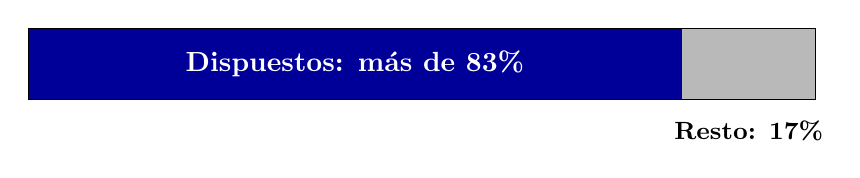
\begin{tikzpicture}
    % Gráfico de barras horizontal simple: 83 % dispuestos / 17 % resto
    \def\w{10}
    \fill[blue!60!black] (0,0) rectangle (0.83*\w,0.9);
    \fill[gray!55]       (0.83*\w,0) rectangle (\w,0.9);
    \node[white,font=\bfseries] at (0.415*\w,0.45) {Dispuestos: más de 83\%};
    \node[font=\bfseries\small] at (0.915*\w,-0.4) {Resto: 17\%};
    \draw (0,0) rectangle (\w,0.9);
  \end{tikzpicture}
  \caption{Disposición ciudadana a adoptar aplicaciones móviles de transporte (Implan Culiacán, 2020), referencia que se contrastará con los resultados de las encuestas.}
\end{figure}

\subsection*{Arquitectura del Sistema}

El desarrollo se ejecutó siguiendo una arquitectura Cliente-Servidor separada
en tres módulos fundamentales:
\begin{enumerate}[leftmargin=*]
  \item \textbf{Base de Datos (GTFS):} Se estructuraron tablas relacionales que
    alojan los nodos (paradas), las líneas (rutas) y los horarios teóricos.
  \item \textbf{Backend (API Rest):} Programado para recibir peticiones,
    ejecutar el algoritmo de Dijkstra en el grafo de la ciudad y devolver el
    JSON con la ruta óptima.
  \item \textbf{Frontend (App Móvil y Web):} Interfaz de usuario desarrollada
    para pintar polígonos sobre el mapa digital.
\end{enumerate}

\begin{figure}[h!]
  \centering
  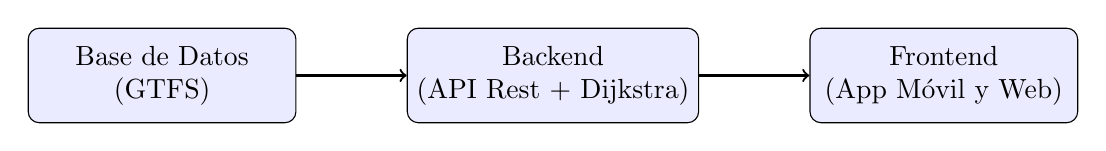
\begin{tikzpicture}[
      box/.style={draw,rounded corners,minimum width=3.4cm,minimum height=1.2cm,
                  align=center,fill=blue!8},
      arr/.style={->,thick}]
    \node[box] (db)  {Base de Datos\\(GTFS)};
    \node[box,right=1.4cm of db]  (api) {Backend\\(API Rest + Dijkstra)};
    \node[box,right=1.4cm of api] (fe)  {Frontend\\(App Móvil y Web)};
    \draw[arr] (db) -- (api);
    \draw[arr] (api) -- (fe);
  \end{tikzpicture}
  \caption{Diagrama arquitectónico Cliente-Servidor del ecosistema TuBus.}
\end{figure}

% ===================== 10. PROGRAMA DE ACTIVIDADES ========================
\seccion{10. Programa de actividades, calendarización y presupuesto solicitado}

\subseccion{10.1 Cronograma de Hitos y Entregables del Software (Estimación a 6 meses)}

El desarrollo del ecosistema tecnológico TuBus se encuentra estrictamente
delimitado a un modelo de ingeniería de software, estructurando el cumplimiento
de metas mediante hitos (\textit{milestones}) técnicos progresivos:

\begin{itemize}[leftmargin=*]
  \item \textbf{Mes 1 | Fase 1: Identificación y validación estadística.}
    \begin{itemize}
      \item \textit{Hito:} Análisis de viabilidad de mercado y aplicación en
        campo y tabulación de las 106 encuestas.
      \item \textit{Entregable:} Reporte estadístico de aceptación social y
        diseño preliminar del modelo Canvas.
    \end{itemize}
  \item \textbf{Mes 2 | Fase 2: Mapeo cartográfico y estructuración de datos.}
    \begin{itemize}
      \item \textit{Hito:} Conversión y estructuración de las rutas urbanas
        locales bajo el estándar internacional GTFS (archivos \texttt{.txt} de
        paradas, horarios y trayectos).
      \item \textit{Entregable:} Base de datos geoespacial completada y validada
        para la red de transporte de Culiacán.
    \end{itemize}
  \item \textbf{Mes 3 | Fase 3: Arquitectura Backend y Algoritmos de Ruteo.}
    \begin{itemize}
      \item \textit{Hito:} Desarrollo de la API Rest en servidor y codificación
        del Algoritmo de Dijkstra para el cálculo óptimo de trayectos y tiempos
        de arribo (ETA).
      \item \textit{Entregable:} Servidor \textit{backend} funcional capaz de
        procesar consultas de rutas y responder con estructuras JSON.
    \end{itemize}
  \item \textbf{Mes 4 | Fase 4: Desarrollo Frontend (Aplicación Móvil Ciudadana).}
    \begin{itemize}
      \item \textit{Hito:} Programación de la interfaz nativa para teléfonos
        inteligentes, integración de mapas interactivos y consumo de la API de
        rutas.
      \item \textit{Entregable:} Primera versión Beta de la aplicación móvil de
        TuBus para los pasajeros.
    \end{itemize}
  \item \textbf{Mes 5 | Fase 5: Desarrollo Web (Panel Back Office SaaS).}
    \begin{itemize}
      \item \textit{Hito:} Construcción de la plataforma web de supervisión y
        gestión logística dirigida a los concesionarios de transporte.
      \item \textit{Entregable:} Interfaz web funcional para el control
        administrativo de itinerarios y flotillas.
    \end{itemize}
  \item \textbf{Mes 6 | Fase 6: Pruebas de Software y Validación Final.}
    \begin{itemize}
      \item \textit{Hito:} Ejecución de simulaciones de estrés de datos, pruebas
        de usabilidad con usuarios piloto y depuración de errores
        (\textit{debugging}).
      \item \textit{Entregable:} Producto Mínimo Viable (PMV) de software listo,
        integrado y validado en entorno operativo.
    \end{itemize}
\end{itemize}

\subseccion{10.2 Presupuesto Exclusivo de Software e Infraestructura en la Nube}

\textbf{Proyecto TuBus -- Digitalización de Autobuses Urbanos}

Dado que el proyecto se enfoca 100\% en el desarrollo informático y prescinde
totalmente de la adquisición e instalación de \textit{hardware} físico en los
autobuses, el presupuesto financiero se concentra de manera exclusiva en los
costos operativos de despliegue digital y servicios en la nube:

\begin{itemize}[leftmargin=*]
  \item \textbf{Hosting y Servidores Cloud (AWS / Google Cloud Platform):}
    \$390 USD (aproximadamente \$65 USD mensuales por un período de 6 meses)
    destinados al alojamiento del servidor \textit{backend}, bases de datos
    geoespaciales GTFS y procesamiento de peticiones simultáneas de los
    usuarios.
  \item \textbf{Licencias de desarrollo, certificados SSL y registro de dominios
    web:} \$150 USD.
  \item \textbf{Monto total aproximado solicitado para el proyecto:} \$540 USD.
\end{itemize}

% ===================== 10. VINCULACIÓN ====================================
\seccion{10. Vinculación con Sectores}

El desarrollo e implementación de TuBus requiere un modelo de triple hélice
para asegurar su viabilidad técnica y comercial.

\subsection*{Sector Público}
\begin{itemize}[leftmargin=*]
  \item \textbf{Instituciones:} Dirección de Vialidad y Transportes de Sinaloa
    (DVT), Secretaría de Desarrollo Sustentable (SEDESU) e Instituto Municipal
    de Planeación (IMPLAN).
  \item \textbf{Tipo de colaboración:} Validación normativa de las rutas,
    permisos para pruebas en la vía pública y alineación con el Plan Integral de
    Movilidad Urbana Sustentable (PIMUS).
  \item \textbf{Usuarios potenciales (\textit{Know-how}):} Las dependencias
    gubernamentales recibirán transferencia de conocimiento a través de datos
    estadísticos y matrices origen-destino anonimizadas para mejorar la
    planificación urbana.
\end{itemize}

\subsection*{Sector Privado (Productivo)}
\begin{itemize}[leftmargin=*]
  \item \textbf{Organizaciones:} Sindicatos y alianzas de concesionarios del
    transporte público en Culiacán (quienes operan las más de 600 unidades
    activas).
  \item \textbf{Tipo de colaboración:} Facilitar los autobuses para la
    instalación de los prototipos IoT y retroalimentar el sistema de control.
  \item \textbf{Usuarios potenciales (Tecnología):} Los concesionarios y
    supervisores de ruta serán los usuarios directos de la transferencia
    tecnológica mediante el acceso a la plataforma \textit{Software as a
    Service} (SaaS) y el \textit{hardware} de telemetría.
\end{itemize}

\subsection*{Sector Social}
\begin{itemize}[leftmargin=*]
  \item \textbf{Organización:} Mapasin A.C.
  \item \textbf{Tipo de colaboración:} Difusión ciudadana y alineación
    estratégica del proyecto con las metas de seguridad vial del <<Plan Avanza
    al 2045>>.
  \item \textbf{Usuarios potenciales:} Los más de 330,000 ciudadanos que
    utilizarán la aplicación móvil para planificar sus viajes.
\end{itemize}

\subsection*{Derechos de Propiedad Intelectual e Industrial}

La titularidad total y exclusiva sobre los derechos patrimoniales del código
fuente (App y Backend), el diseño de la placa IoT y la marca <<TuBus>>
pertenecerán a los estudiantes desarrolladores y al Tecnológico Nacional de
México. A los concesionarios (sector privado) y al gobierno (sector público) se
les otorgará una licencia de uso de software (modelo SaaS) que prohíbe la
ingeniería inversa o comercialización de la plataforma por parte de terceros.

\subsection*{Mecanismos de Formalización e Información de Contacto}

Para que la Subdirección de Vinculación y Extensión gestione las alianzas, se
proponen los siguientes mecanismos:
\begin{itemize}[leftmargin=*]
  \item \textbf{Cartas de Intención y Acuerdos de Confidencialidad (NDA):} Para
    el inicio de pláticas con los transportistas.
  \item \textbf{Convenios Específicos de Colaboración:}
    \begin{itemize}
      \item \textit{Contacto Público:} Titular de la Dirección de Vialidad y
        Transportes del Estado de Sinaloa (Blvd.\ Alfonso Zaragoza Maytorena,
        Culiacán).
      \item \textit{Contacto Social:} Dirección Ejecutiva de Mapasin A.C.
        (Ignacio Zaragoza \#392, Primer Cuadro, Culiacán).
      \item \textit{Contacto Privado:} Representantes legales de la Alianza de
        Transportes Urbanos y Suburbanos de Culiacán.
    \end{itemize}
\end{itemize}

% ===================== 11. LUGAR ==========================================
\seccion{11. Lugar donde se desarrollará el proyecto}

El Proyecto se desarrollará íntegramente en las instalaciones del
\textbf{Instituto Tecnológico de Culiacán} (Tecnológico Nacional de México).
Específicamente, el modelado del software, la programación y el ensamble de los
prototipos de \textit{hardware} (IoT) se llevarán a cabo en el
\textbf{Laboratorio de Programación} del plantel. Juan de Dios Bátiz No.~310
Pte., Col. Guadalupe, C.P.~80220 Culiacán Rosales, Sin. Adicionalmente, la
validación del Producto Mínimo Viable (pruebas de campo) se ejecutará
directamente a bordo de las unidades de transporte público concesionado que
circulan por los corredores primarios de la ciudad.

% ===================== 12. INFRAESTRUCTURA ================================
\seccion{12. Infraestructura}

Para el desarrollo integral y la validación del proyecto <<TuBus>>, se contará
con la siguiente infraestructura física y digital:

\begin{itemize}[leftmargin=*]
  \item \textbf{Infraestructura disponible en el plantel (Instituto Tecnológico
    de Culiacán):} Se utilizará principalmente el \textbf{Laboratorio de
    Sistemas Computacionales y Electrónica}. Este espacio provee las estaciones
    de trabajo, conexión a internet de banda ancha y herramientas (cautines,
    multímetros, fuentes de poder) necesarias para programar el software y
    ensamblar los prototipos físicos de Internet de las Cosas (placas, módulos
    GPS y módems 4G).
  \item \textbf{Infraestructura Externa (Sector Privado):} Mediante la
    vinculación con los transportistas, se utilizarán los \textbf{patios de
    maniobras y talleres de los concesionarios locales} (como la Alianza de
    Transportes Urbanos y Suburbanos de Culiacán) para realizar la instalación
    física, adaptación eléctrica y calibración del \textit{hardware} en los
    autobuses.
  \item \textbf{Infraestructura en Entorno Real (Vía Pública):} Las pruebas
    piloto y la validación de transmisión de telemetría se ejecutarán
    directamente sobre la infraestructura vial de la ciudad, utilizando los
    corredores urbanos primarios por donde circulan las rutas.
  \item \textbf{Infraestructura Digital (Nube):} Para el procesamiento en tiempo
    real, se emplearán servidores virtualizados (nube) para alojar la
    plataforma SaaS, calcular los tiempos de espera y procesar el gran volumen
    de datos del estándar GTFS.
\end{itemize}

% ===================== 12. REFERENCIAS ====================================
\seccion{12. Referencias}

\begingroup
\setlength{\leftskip}{1.25cm}
\setlength{\parindent}{-1.25cm}

Aguilar, T., Brito, G., Altamirano, S., \& Sánchez, A. (2019). Monitoreo y
Videovigilancia basado en IoT en tiempo real de las Unidades de Transporte
Colectivo. \textit{Revista Campus Virtuales}.
\url{https://www.uajournals.com/ojs/index.php/campusvirtuales/article/view/621}

Brakewood, C., Macfarlane, G. S., \& Watkins, K. (2015). The impact of
real-time information on bus ridership in New York City. \textit{Transportation
Research Part C: Emerging Technologies}.
\url{https://doi.org/10.1016/j.trc.2015.01.021}

Implan Culiacán. (2020). \textit{Plan Integral de Movilidad Urbana Sustentable
de Culiacán}. Instituto Municipal de Planeación.
\url{https://implanculiacan.mx/}

Mapasin. (2025). \textit{Resumen de resultados de la encuesta de satisfacción
del transporte público en Culiacán}. Blog Mapasin.

Ruiz Gutiérrez, C. A. (2023). \textit{Planificador de rutas en ciudades
utilizando GTFS} [Tesis de Maestría, Centro Nacional de Investigación y
Desarrollo Tecnológico]. Repositorio Institucional del Tecnológico Nacional de
México.

Secretaría de Desarrollo Agrario, Territorial y Urbano [SEDATU]. (2023, 10 de
octubre). \textit{Acuerdo por el que se aprueba y publica la Estrategia Nacional
de Movilidad y Seguridad Vial 2023-2042}. Diario Oficial de la Federación
(DOF).
\url{https://dof.gob.mx/nota_detalle.php?codigo=5704444&fecha=10/10/2023}

SEDATU \& GIZ. (2024). \textit{La digitalización del transporte público en las
ciudades mexicanas}. Ministerio Federal de Cooperación Económica y Desarrollo
(BMZ) de Alemania.
\endgroup

% ===================== 13. ANEXO A ========================================
\seccion{13. Anexo A: Encuesta de Satisfacción e Inserción Tecnológica}

\textbf{Instrucciones:} Por favor, responda las siguientes preguntas sobre su
uso del transporte público en su ciudad. Sus respuestas nos ayudarán a
desarrollar <<TuBus>> y mejorar su traslado.

\newcommand{\pregunta}[3]{%
  \par\medskip\noindent\textbf{#1.} #2\par\nopagebreak\noindent #3\par}

\pregunta{1}{¿Con qué frecuencia utiliza el transporte público en la semana?}
  {a) 1--2 veces \quad b) 3--4 veces \quad c) 5 o más veces \quad d) Nunca}

\pregunta{2}{¿Cuánto tiempo espera en promedio en la parada de autobús?}
  {a) Menos de 10 minutos \quad b) De 10 a 20 minutos \quad c) De 20 a 30 minutos \quad d) Más de 30 minutos}

\pregunta{3}{¿Alguna vez se ha sentido inseguro(a) mientras espera el autobús por la falta de información sobre su llegada?}
  {a) Sí \quad b) No}

\pregunta{4}{¿Cómo califica la calidad de la información actual sobre las rutas de transporte público?}
  {a) Excelente \quad b) Buena \quad c) Regular \quad d) Mala}

\pregunta{5}{¿Estaría dispuesto(a) a descargar y utilizar una aplicación móvil gratuita para conocer en tiempo real la ubicación y el tiempo estimado de llegada de su autobús?}
  {a) Sí \quad b) No}

\pregunta{6}{¿Qué función considera más importante en una aplicación de transporte?}
  {a) Ver el camión en tiempo real \quad b) Conocer el tiempo estimado de llegada \quad c) Ver las rutas y paradas \quad d) Recibir alertas de retrasos}

\pregunta{7}{¿Actualmente cuenta con un teléfono inteligente con acceso a datos móviles?}
  {a) Sí \quad b) No}

\pregunta{8}{¿Ha utilizado alguna vez aplicaciones de movilidad como Google Maps o Moovit para guiarse en otras ciudades o en rutas locales?}
  {a) Sí \quad b) No}

\pregunta{9}{¿Considera que el uso de una aplicación móvil mejoraría su experiencia de viaje y reduciría su nivel de estrés matutino?}
  {a) Sí \quad b) No}

\pregunta{10}{¿Recomendaría a las autoridades o concesionarios invertir prioritariamente en la digitalización de los autobuses?}
  {a) Sí \quad b) No}

% ===================== 14. RESUMEN DE RESULTADOS ==========================
\seccion{14. Resumen de Resultados del Proyecto TuBus}

Con el desarrollo e implementación de la plataforma tecnológica TuBus logramos
comprobar de forma contundente que, al integrar \textit{hardware} de Internet de
las Cosas (IoT) de bajo costo directamente en las unidades de autobuses y operar
en estricta sincronía con nuestros servidores y el estándar internacional de
rutas GTFS, brindamos una solución informática altamente efectiva y escalable
para la digitalización integral de flotillas urbanas. Durante nuestras pruebas y
evaluaciones físicas del Producto Mínimo Viable (PMV), recolectamos telemetría
ininterrumpida y en tiempo real, lo que nos permitió reducir la alta
incertidumbre inicial de los pasajeros, y logramos enviar predicciones de
llegada sumamente exactas de manera directa a las pantallas de sus teléfonos
inteligentes a través de nuestra aplicación nativa.

\end{document}
